\subsubsection{\Extent}\label{ssec:designdims:extent}

\begin{figure}[t]
  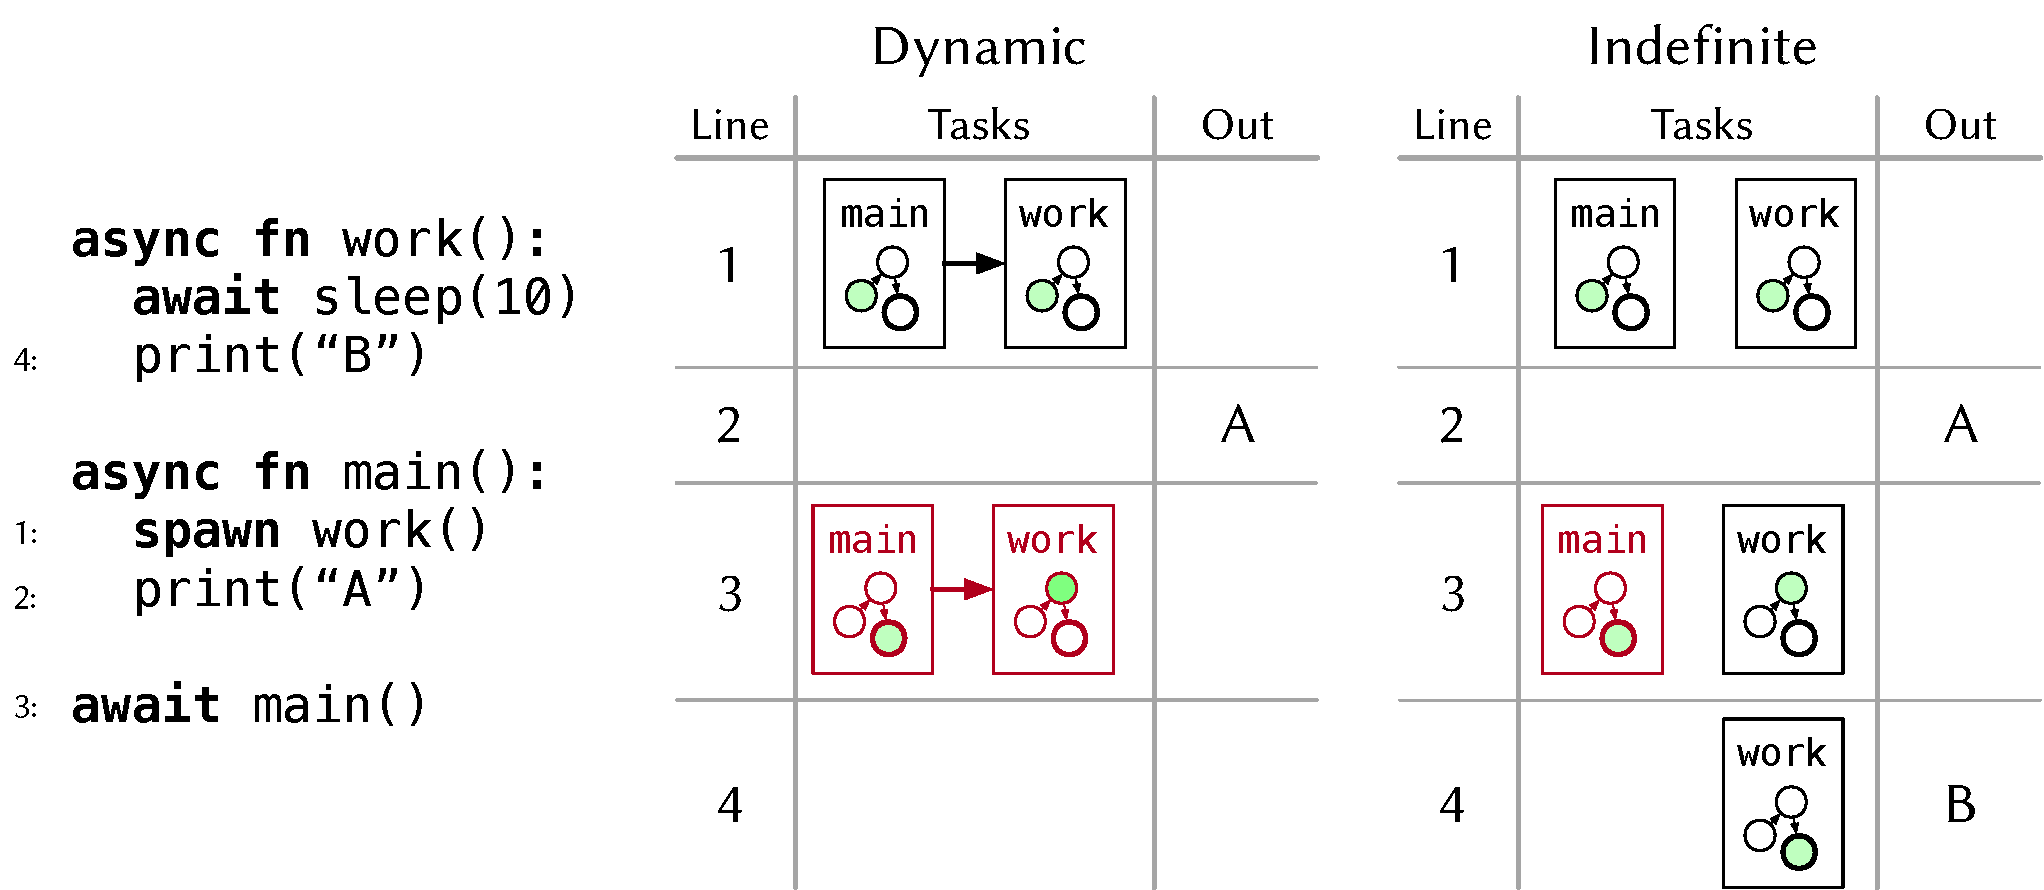
\includegraphics[width=0.82\linewidth]{./f/extent.pdf}
  \caption{An example program demonstrating the \extent dimension, executed with Swift (\dyn) and \Js (\indef). Each column shows the task structure and output after executing each line. Arrows between tasks indicate a parent-child relationship used for \dyn \extent.}
  \label{fig:extent}
\end{figure}

% \begin{figure}[t]
%   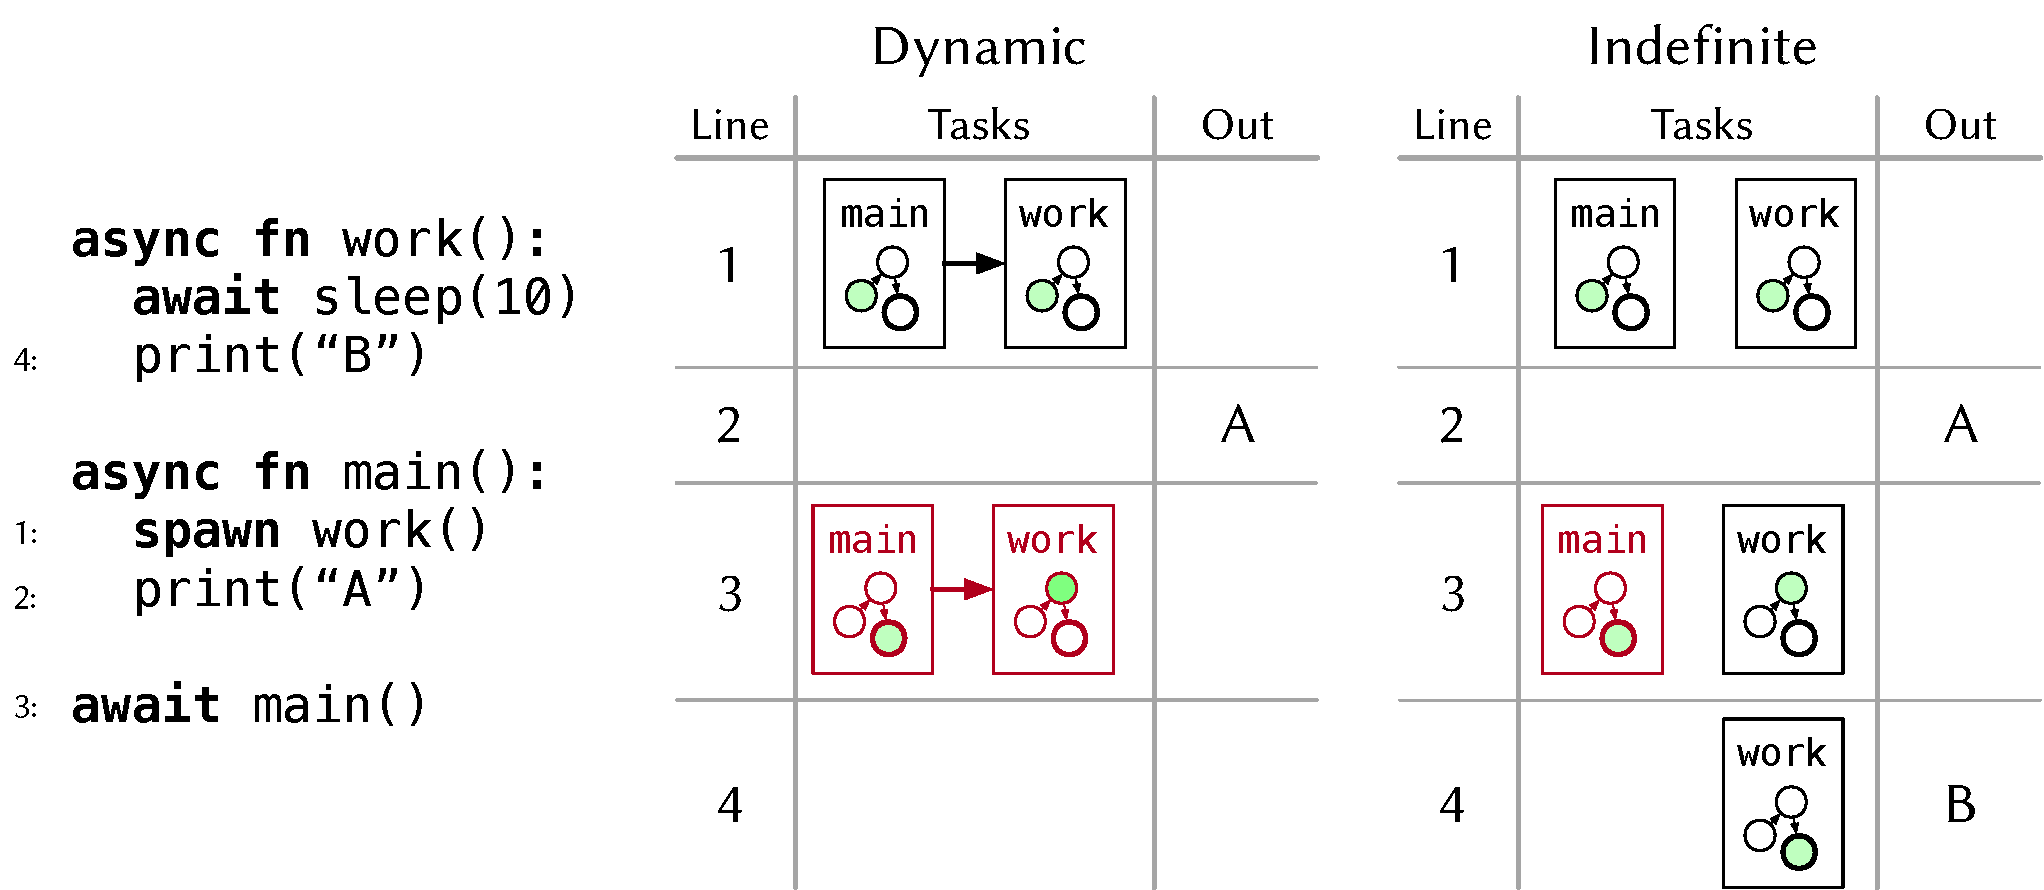
\includegraphics[width=0.7\linewidth]{./f/extent.pdf}
%   \caption{An example program demonstrating the \extent dimension, executed with Swift (\dyn) and \Js (\indef). Each column shows the task structure and output after executing each line. Arrows between tasks indicate a parent-child relationship used for \dyn \extent.}
%   \label{fig:extent}
% \end{figure}

Borrowing terminology from the Lisp community, the \extent of a task is the interval of time during which that task is capable of executing. For example, consider the program in \Cref{fig:extent}. What is the extent of the \code|spawn child_work()| task? The answer is it depends on quite a number of factors, as previously illustrated in \Cref{fig:motivating-example}.

In some designs for straight-line asynchrony, especially earlier designs, tasks by default have an \indef \extent: the task can live until it is no longer reachable, at which point the task is destructed. \Js, \CSharp, Python+Asyncio, and Rust+Tokio/Smol all use \indef \extent. Note that designs differ on how to determine reachability (see \Cref{ssec:designdims:references}), and designs also differ on the mechanism for destruction (see \Cref{ssec:designdims:destruction}). \Cref{fig:extent} illustrates \indef \extent, showing how the \code|child_work()| task outlives its parent \code|parent_work()| task, and the program waits until the work is completed.

Some have called \indef \extent an ``unstructured'' approach to asynchrony~\cite{smith_thoughts_2016}, akin to using goto for control flow, as task handles can easily go unhandled, leaving asynchronous work dangling with no clear policy for managing it.
%
This line of thought has led to the devleopment of ``structured'' asynchrony approaches~\cite{sustrik_structured_2025,mccall_swift_2021,elizarov_kotlin_2021}, which we describe as having \dyn \extent, found in Swift and Python+Trio. With \dyn \extent, a task's extent is tied to the extent of another task. In \Cref{fig:extent}, under \dyn \extent, the \code|child_work()| task is associated with the \code|parent_work()| task. When the \code|parent_work()| task completes, its associated tasks are destructed, which means cancellation in the case of Swift. Therefore the second print never occurs.

\paragraph{Design rationale.}

The main argument for \dyn \extent is that limiting tasks to known scopes leads to programs that are easier to reason about, and compose better with other language features~\cite{mccall_swift_2021,elizarov_kotlin_2021}. For instance in Python, \dyn \extent can ensure that a task within a \code|with| block will not use resources (e.g., file descriptors) after they have been cleaned up~\cite{smith_thoughts_2016}. However, existing implementations of \dyn \extent only support a strictly hierarchical model of parent-child task relationships (via \code|TaskGroup| in Swift and \code|Nursery| in Trio). These implementations disallow programs that might have more complex dependencies between tasks, such as two parent tasks awaiting the same child task.
